\chapter{Problemanalyse}

    I det følgende kapitel vil rapporten gennemgå problemanalysen, hvor der  ses nærmere på hvad Internet of Things er og hvilke sikkerheds aspekter der er ved IoT og hvordan disse kan udnyttes.
    
    \section{Internet of Things}
        Begrebet Internet of Things (IoT) blev skabt i 1999 af MIT Auto-ID Center grundlæggere, Kevin Ashton og David L. Brock.\autocite{Hashmi2017} Auto-ID er en bred vifte af teknologier brugt i industrier til at øge effektiviteten, automation samt reduktion af fejl. Disse teknologier kan være sensorer, stemme genkendelse, stregkode osv.
        Siden 2003 har Auto-ID teknologi ændret sig til hovedsageligt at være Radio Frequency Identification(RFID) fra sensore, stemme genkendelse og stregkoder osv.\autocite{Sundmaeker2010}. Oprindeligt var MIT Auto-ID Center industri sponsoreret forsknings og udviklingscenter, hvor alt deres arbejde blev frit tilgængeligt. Centerets vision var:\\
        \textit{``The Auto-ID Center envisions a world in which all electronic devices are networked and every object, whether it is physical or electronic, is electronically tagged with information pertinent to that object.''} -\autocite[Kapitel 2,p. ~4]{Sarma2001} Visionen var altså at det var muligt at forbinde alle fysiske objekter til et netværk. 
        I oktober 2003 skiftede MIT Auto-ID Center navn til Cambridge Auto-ID Lab og blev lukket. Centeret blev delt i Auto-ID Labs forsknings enhed og EPCglobal kommercielt enhed eget af UCC og EAN.\autocite{Sundmaeker2010}\\
        Formålet med Auto-ID Labs i dag er at udvikle et netværk, som forbinder computere til objekter. Objekterne er ikke blot hardware eller software som er forbundet på et netværk, men alt hvad der benyttes til at skabe IoT. Det vil sige hardware, netværk software og protokoller, sprog til at beskrive objekter, således at computer kan kommunikere. Det er ikke et nyt internet, men elementer bygget oven på eksisterende internet teknologi, som gøre det muligt at spore og dele information på tværs af internettet.\autocite{Sundmaeker2010} \\
        \begin{figure}[H]
            \centering
                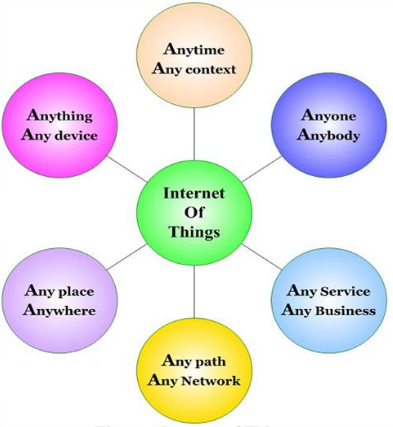
\includegraphics[width=0.55\textwidth]{figures/IoT_definition.png}
            \caption{IoT kommunikation.\autocite{Sundmaeker2010}}\label{fig:IOTkom}
        \end{figure}
        Ved at overveje det nævnte kan IoT-enheder defineres som enheder eller ting, som gennem trådløse forbindelser samt kabelforbindelser i et netværk er i stand til at samarbejde med hinanden, uden at skulle bruge det menneskelige element i kommunikationen, se figur \ref{fig:IOTkom}. IoT-enhederne er i stand til at skabe flydende kommunikation.\autocite{Hashmi2017}
        IoT-enheder kan have følgende kommunikations mønstre: menneske til enhed, enhed til enhed.\\
        Dette vil altså sige at IoT-enheder kan defineres som alt fra General Purpose Devices (Computere, printere, mobiltelefoner eller lignende) (GPD) til kaffemaskiner og toiletter tilkoblet WI-FI eller Ethernet. Da GPD enheder er produceret af firmaer som Apple, HP, Samsung og Lenovo, er disse ofte produceret med kundernes sikkerhed i fokus. Rapporten har på baggrund af dette valgt at ekskludere GPD enheder fra rapportens arbejdsområde, da disse ofte får software opdateringer der øger sikkerheden på produkterne.
        Arbejdsområdet indenfor IoT er altså reduceret til at være fokuseret på de produkter der kun nyligt er kommet på markedet, så som kaffemaskiner og toiletter med internet funktioner. \\
